\documentclass{article}
\usepackage[table]{xcolor}
\usepackage{tikz,booktabs,graphicx}
\definecolor{tabbg}{gray}{0.98}
\definecolor{header}{RGB}{30,60,120}
\begin{document}
Legitimate uses of white text, near-white backgrounds, phantoms and low opacity.
\begin{table}[h]
\centering
\begin{tabular}{lrr}
\toprule
\rowcolor{header}\textcolor{white}{\textbf{Method}} & \textcolor{white}{\textbf{Recall}} & \textcolor{white}{\textbf{QPS}} \\
\midrule
\rowcolor{tabbg} Baseline & 0.90 & \phantom{0}950 \\
Ours & 0.95 & 1200 \\
\bottomrule
\end{tabular}
\caption{A table with a dark header and light row shading.}
\end{table}
Alignment: \phantom{Baseline method}aligned text. \hphantom{000}padded.
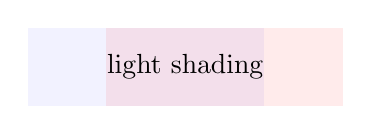
\begin{tikzpicture}
\fill[blue,opacity=0.05] (0,0) rectangle (3,1);
\fill[red,fill opacity=0.08] (1,0) rectangle (4,1);
\node at (2,0.5) {light shading};
\end{tikzpicture}
\scalebox{0.5}{half-size but readable}
\end{document}
